%%------------------------------------------------------
% 
%% UNIVERSIDADE FEDERAL DE SANTA CATARINA - UFSC
%
%% Prof.: Wyllian B. da Silva
%%
%% Template: estilo IEEEtran [paper com duas colunas]
%% Adaptado de: https://ieeeauthorcenter.ieee.org/create-your-ieee-article/use-authoring-tools-and-ieee-article-templates/ieee-article-templates/templates-for-transactions/
%               https://ctan.org/tex-archive/macros/latex/contrib/IEEEtran?lang=en

%% Instruções: http://mirrors.ctan.org/macros/latex/contrib/IEEEtran/IEEEtran_HOWTO.pdf
%%
%% Recomendações:
%% Utilize o Edito Kile (SO Linux)
%% Certifique-se de que a codificação de caracteres utilizada é a UTF-8





\documentclass[journal]{IEEEtran}


%%------------------------------------------------------
%% Packages
%%------------------------------------------------------
\usepackage[T1]{fontenc}           %% Codificação de caracteres
\usepackage[utf8]{inputenc}        %% Codificação de caracteres (conversão automática dos acentos)
\usepackage[dvips]{graphicx}       %% para a macro includegraphics 
\usepackage[english,brazil]{babel} %% PT_BR e EN (o último define a prioridade no arquivo)
\usepackage{pgf}                   %% macro para criar gráficos
\usepackage{epsfig}                %% or use the epsfig package if you prefer to use the old commands
\usepackage{graphics}              %% use the graphics package for simple commands
\usepackage{graphicx}              %% or use the graphicx package for more complicated commands
\usepackage{epstopdf}              %% enable EPS (convert to PDF)
\usepackage{float}                 %% float environment
\usepackage{eqparbox}              %% to define a group of boxes 
\usepackage{hyphenat}              %% prevent hyphenation
\usepackage{hyperref}              %% enalbe one-click link

% \usepackage{showframe} %% just for the example

% \usepackage[sort,compress]{cite} %% disable if natbib package is activated
\usepackage[numbers,sort&compress,square]{natbib} %% e.g., [2-5]



%%------------------------------------------------------
%% Definitions
%%------------------------------------------------------

\hyphenation{op-tical net-works semi-conduc-tor}

%% Can use something like this to put references on a page
%% by themselves when using endfloat and the captionsoff option.
\ifCLASSOPTIONcaptionsoff
  \newpage
\fi


%%----------------- Definindo as variáveis com números
\makeatletter
%
\newcommand{\prenome}{\afterassignment\prenome@aux\count0=}
\newcommand{\prenome@aux}{\csname prenome\the\count0\endcsname}
%
\newcommand{\nomedomeio}{\afterassignment\nomedomeio@aux\count0=}
\newcommand{\nomedomeio@aux}{\csname nomedomeio\the\count0\endcsname}
%
\newcommand{\sobrenome}{\afterassignment\sobrenome@aux\count0=}
\newcommand{\sobrenome@aux}{\csname sobrenome\the\count0\endcsname}
\makeatother
%%%%%

%%----------------- Configurações de hyperlinks
%% Não decorado, sem destaque
\hypersetup{
  colorlinks=false,
  pdfborder={0 0 0},
}




%%------------------------------------------------------
%% Configurações
%%------------------------------------------------------

%%----------------- Título
\title {Dance Dance Revolution}

\newcommand{\emailautor}                              {seuemail@grad.ufsc.br}

\newcommand{\siglaRevista}{UFSC}

\newcommand{\Revista}{Universidade Federal de Santa Catarina (UFSC)}

% %%----------------- Vários Autores
\author{\authorblockN{\prenomePrincipal\nomedomeioPrincipal\sobrenomePrincipal~\authorrefmark{Jéssica Santos Borges} e
\prenome2\sobrenome2\authorrefmark{Leticia Meurer} \membership
% 
\\\IEEEauthorblockA{\IEEEauthorrefmark{1}Universidade Federal de Santa Catarina (UFSC)}
% 
}}

%%------------------------------------------------------
%% Abstract
\IEEEtitleabstractindextext{

  {\selectlanguage{brazil}
    \begin{abstract}
     Este relatório tem como objetivo apresentar a formação de um jogo em terminal utilizando a linguagem C de programação. Nele estão contidos os problemas encontrados para execução e os métodos utilizados para que fosse possível formar uma adaptação de Dance Dance Revolution.
    \end{abstract}
    %%----------------- Keywords
    \renewcommand\IEEEkeywordsname{Palavras-chave} 
   \begin{IEEEkeywords}
    Programação, linguagem C, jogo de Arcade.
    \end{IEEEkeywords}
  }

  {\selectlanguage{english}
    \begin{abstract}
    This report aims to present the formation of a game in terminal using the C programming language. In it are contained the problems encountered for execution and the methods used so that it was possible to form an adaptation of Dance Dance Revolution. 
    \end{abstract}
    %%----------------- Keywords
    \begin{IEEEkeywords}
    Programming, C language, Arcade game.
    \end{IEEEkeywords}
  }
}


\begin{document}



%%%%%%%%%%%%%%%%%%%%%%%%%%%% Inserção de informações
\maketitle
\IEEEdisplaynontitleabstractindextext
\IEEEpeerreviewmaketitle


%%%%%%%%%%%%%%%%%%%%%%%%%%% SECTION INTRODUÇÃO
\section{Introdução}

\IEEEPARstart{E}{ste} projeto tem como intuíto realizar uma atividade prática que utilize os conhecimentos adquiridos durante as aulas para a implementação de um jogo em terminal. Assim,  utilizou-se do sistema operacional Ubunto e a linguagem C.

Teve-se como inspiração o antigo jogo de Arcade lançado em 1998 no Japão - Dance Dance Revolution (Figura 1), no qual, os jogadores devem acertar as setas em sequência conforme as mesmas aparecem na tela. Existem algumas variações deste jogo, no entanto, todos seguem a mesma ideia.

\begin{figure}[h]
    \centering
    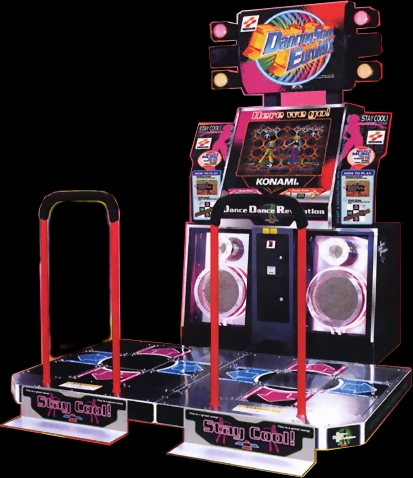
\includegraphics[width=.3\textwidth]{dsem.png}
    \caption{Dance Dance Revolution (1998) - Fonte: Emuparadise (2019).}
    \label{fig:dsem}
\end{figure}

A elaboração do relatório tem por objetivo discutir a realização do jogo para um único usuário. Primeiramente realizou-se uma verificação de todos os pontos que precisavam ser melhorados como o layout inicial, a distribuição da setas e a inclusão de tempo. Após isso, realizou-se um levantamento de problemas, tendo como o maior deles o ajuste da música de fundo.

%%%%%%%%%%%%%%%%%%%%%%%%%%%%%%%%%%%%% Subsection
\subsection{Problemas}
Nesta subseção serão apresentados alguns problemas encontrados para elaboração do jogo como um todo e suas possíveis resoluções.

%%%%%%%%%%%%%%%%%%%%%%%%%%%%%%%%%%%% Subsubsection

\subsubsection{Música}
um dos problemas encontrados foi a implementação de música no decorrer da atividade, o qual gerou uma série de erros. Primeiramente a música tocava inteira e só iniciava-se o jogo quando a música chegava ao fim, depois o jogo começava e a música só se iniciava quando o mesmo terminava. Uma das maiores dificuldades foram encontrar soluções simples e eficientes para o ajuste nos problemas. 
 
Para que a música e jogo ocorressem ao mesmo tempo, foi adicionado o símbolo ''\&'' a função \textit{"play \%s(nome da música.extensão) -q \&"} o que permitiu que ambos funcionassem corretamente porém, a música continua a tocar mesmo com o término do jogo, criando assim um novo erro. 

O problema por fim foi solucionado pela adaptação da função \textit{kill}, a \textbf{pkill}, que tem por finalidade interromper a parte desejada do código, o que neste caso, utilizou-se para encerrar a música juntamente com o terminar do jogo. 

No decorrer do trabalho serão apresentados a metodologia utilizada para criação do jogo, seguida pelos resultados encontrados durante a execução, a conclusão e o apêndice, onde encontra-se o código de criação do jogo.


%%%%%%%%%%%%%%%%%%%%%%%%%%%%%%%%%%% Section
\section{Metodologia}
O jogo utiliza quatro bibliotecas distintas e diversas funções e ponteiros localizados dentro da biblioteca \textbf{funcoes\_jogo}. Nela, econcontram-se todos códigos utilizados. 

Localizada dentro da pasta \textbf{code}, utiliza-se o código \textbf{main} para inserir duas funções. A \textbf{startmenu}, que tem como finalidade abrir a tela inicial do jogo, proporcionar a cor preta no fundo de tela, a cor vermelha empregada na alteração de cor das setas, e as cores azul, verde e branca na mudança dos emojis apresentados conforme os moviemento são executados corretamente. A função \textbf{gameview} tem como principal utilidade a formação do código, as strings (setas), emojis, ponteiros, if, while e o chamamento das demais funções utilizadas no decorrer da criação do jogo. 

Existem algumas funções aplicadas e chamadas pela função descrita anteriormente, como a \textbf{play\_sound} que emprega o play para a inserção de música de fundo, o qual está situado dentro da pasta SOX que serve como ferramenta para a linha de comando. A função \textbf{lose\_winview} que tem por objetivo auxiliar na melhor funcionalidade do jogo, permitindo que ao chegar em determinada pontuação o usário vença ou no caso de o mesmo errar a coordenada, ele perca.

A maior biblioteca utilizada para execução do jogo é a \textbf{ncurses} que possibilita o uso de cores, a introdução de janelas e o uso do teclado para efetuar os movimentos necessários. A bilioteca \textbf{stdio} que serve para entrada e saída do teclado. A \textbf{stdlib} tem como finalidade acessar pastas e mover diretórios internos. E, utilizando a biblioteca \textbf{time}, pôde-se acrescentar tempo para as jogadas ocorrerem.

O gerenciamento lógico do jogo consiste principalmente em setas e funções que realizam a diferenciação de cores das mesmas para o vermelho e são representadas pelas teclas W, S, A e D. O jogador tem um tempo máximo de até 5s para realizar uma próxima atividade, assim, se o mesmo se ausentar por mais tempo o jogo se encerra e uma nova partida precisa ser iniciada.

Ao atingir determinada pontuação durante uma sequência de acertos na partida, o jogador automaticamente é transferido para um nível superior e passa a receber pontuações maiores, o que é gerenciado pelo ponteiro \textbf{*prt\_nivel}.

Para que haja um vencedor ou um perdedor durante a partida adicionou-se o ponteiro \textbf{*prt\_pontos}, que possibilita as diferentes pontuações serem atribuidas para cada movimento feito pelo usuário, assim, seu \textit{score} varia de acordo com seus acertos, erros e mudanças de níveis. 

%%%%%%%%%%%%%%%%%%%%%%%%%%%%%%%%%%%% Section
\section{Resultados}

O template inicial é formado pelas explicações de como o jogo funciona, diversos caracteres formando o nome do mesmo e o play, como pode ser observado na figura 2.

\begin{figure}[h]
    \centering
    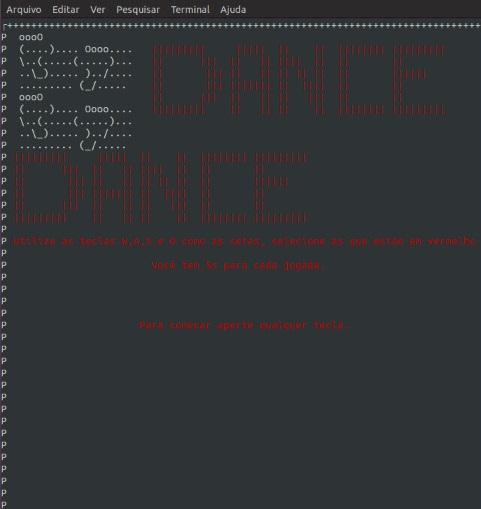
\includegraphics[width=.4\textwidth]{template.jpeg}
    \caption{Template inicial.}
    \label{fig:template}
\end{figure}

A parte gráfica do jogo é composta por setas: uma para cima (W), uma para baixo (S), uma para esquerda (A) e outra para direita (D) alocadas em uma única coluna, como pode ser observado na figura 3. 

O objetivo era colocar todas em forma de teclado, alinhando a seta direita com a esquerda, o que não pode ser alcançado devido a um movimento incompreendido da string, o qual movia apenas o início da mesma e o restante ficava no mesmo lugar.

\begin{figure}[h]
    \centering
    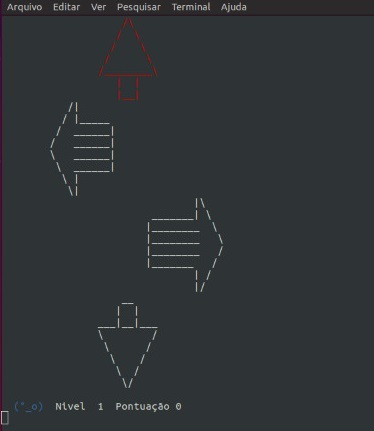
\includegraphics[width=.3\textwidth]{SETAS.jpeg}
    \caption{Formação gráfica.}
    \label{fig:setas}
\end{figure}

Os resultados esperados após a formação do jogo são de aproveitamento dos usuários e entendimento de todas as posições atribuídas. Juntamente com o funcionamento de todas a partes ao mesmo tempo, como as setas trocando de cor para identificação, a música tocando em tempo correto e as pontuações geradas adequadamente.

%%%%%%%%%%%%%%%%%%%%%%%%%%%%%%%%%%%% Section
\section{Conclusão}
Conforme o exposto, pode-se concluir que o objetivo principal do jogo, de ter todas as peças funcionando corretamente e ao mesmo tempo, foram alcançados. Com o desenvolvimento deste projeto foi possível ter um maior entendimento da linguagem C e colocar em prática todo o assunto verificado em teoria na sala de aula. Para projetos futuros, o que não foi possível implementar neste, teríamos um personagem executando os movimentos ao invés de flechas de indicações para o movimento.  

%% Appedix (if necessary)
\appendices

%%----------------- Apêndice
\section{Músicas utilizadas}
Up in my jam. 
\\<https://www.audiolibrary.com.co/kubbi/up-in-my-jam-all-of-a-sudden. Acesso em: Junho de 2019.>

Family crownd celebration. \\<https://www.youtube.com/audiolibrary/soundeffects?ar=3. Acesso em: Junho de 2019.>

Leszek\_Szary 
\\<https://freesound.org/people/Leszek\_Szary/sounds/171672/. Acesso em: Junho de 2019.>

%%%%%%%%%%%%%%%%%%%%%%%%%%% References (Option 2): incorporeted
 \begin{thebibliography}{10} 
 
   \bibitem{dosSantos:2003}
     dos Santos, L. B., \emph{Utilizando a biblioteca NCURSES}, Rio de Janeiro: Viva o Linux, 2003. pp. 4.
 
   \bibitem{Pinheiro:2012} 
     Pinheiro, F. A. C., 2012. {\em Elementos de programação em C.} Porto Alegre: Bookman, 2012. 
     978-85-407-0202-8.

   \bibitem{da Silva:2019} 
     da Silva, W. B. 2019. In: {\em CPF}, Curitiba. <https://github.com/wyllianbs/CPF>.
 
 \end{thebibliography}



\end{document}